#

\documentclass[10pt,journal,compsoc]{IEEEtran}

% \usepackage{cite}
\usepackage[pdftex]{graphicx}
\usepackage{natbib}
%\usepackage{url}
\usepackage{hyperref}
 \usepackage{breakurl}

 \usepackage{xspace}
\newcommand{\ie}{\emph{i.e.,}\xspace}
\newcommand{\eg}{\emph{e.g.,}\xspace}
\newcommand{\ea}{\emph{et al.}\xspace}
\newcommand{\cv}{COVID-19\xspace}
\newcommand{\tool}{COVID-19 Analysis Tools\xspace}


% \newcommand{\cm}[1]{\textbf{#1}}

\begin{document}

\title{Data Visualization for the Understanding of \cv}



\author{%
	João L. D. Comba
	\IEEEcompsocitemizethanks{
	\IEEEcompsocthanksitem João L. D. Comba is at Instituto de Informática, UFRGS, Brazil.\protect
}}


\IEEEtitleabstractindextext{%
\begin{abstract}
Visualization techniques have been front-and-center in the efforts to communicate the science around COVID-19 to the very broad audience of policy makers, scientists, healthcare providers, and the general public. In this paper I summarize and illustrate with examples how visualization can help understand different aspects of the pandemic.  \end{abstract}
}


% make the title area
\maketitle

%Up to 2,500-3,000 words in length, including the abstract, references, bios, figures, and all other text in the article.  When counting words, note that tables and figures should be counted as 250 words each.

%\section*{First Approaches to visualize \cv data}

The deadly impact of \cv is driving a massive amount of research that aims at understanding the various characteristics of the pandemic. While there is no vaccine, considerable effort has been devoted to understanding the spread of the disease in different places in the world. The speed with which the disease has spread throughout the world demands agile solutions to understand and estimate the disease progression.

Interactive \emph{dashboards} with several charts surfaced in different formats to offer concise ways to express the pandemic's growth. Fig.~\ref{fig:dashboards} illustrates some examples. The dashboard developed by Johns Hopkins University (JHU)~\cite{dashboardJHU} was the first to track and display information on case and death totals for different countries and states in the United States. Along with lists of total counts and histograms, a \emph{bubble map} composed of circles of different radii allows a visual inspection of how serious the pandemic is around the world. Interesting plots were created on news outlets such as the New York Times (NYT)~\cite{NYT,WP} and the Washington Post~\cite{WP}. For example, NYT used \emph{Choropleth maps}, a representation where geographical regions (countries or states) are mapped to colors associated with a measurement for that region (\eg number of cases). This representation is useful to communicate trends, such as the average daily counts for the past week. Similarly, they display the time series evolution for each region using \emph{line heatmaps}, where daily values are mapped to colors and displayed in a row.
Our work (described in more detail below) used both Choropleth maps and line heatmaps in the development of dashboard specially designed for Brazil. Using a focus-plus-context interface with coordinated views, the user can inspect the context using two Choropleth maps (one for the states and a second for a state selected), as well as details using two \emph{matrix heatmaps} (collection of stacked line heatmaps) for states and cities. The tool displays daily or cumulative data, absolute or relative to population, and supports filtering by a time interval.

%
A vast collection of community-developed dashboards and interactive tools about \cv are available. Good starting places to look are the data hub hosted by Tableau and the top 100 R resources organized by Soetewey~\cite{R-resources}. In-depth analysis is available at sites such as \emph{Our World in Data}\cite{OWID},  \emph{Bing}~\cite{BING} and the \emph{COVID Tracking Project}~\cite{COVID-TRACKING}, among others. After developing the Brazilian dashboard, we devoted our efforts to create a set of tools to compare the spread of \cv data in different regions of the world~\cite{covid19-tools}. We collected data from more than 6,000 locations in the world, and our interface has different charts that support visualizing multiple locations in a single chart. Since the pandemic is at different stages in the world, we allow the user to align the time-series of data by a certain data the series passes a given threshold (\eg after 100 cases). This representation is useful to observe when different locations passed through specific checkpoints (top of Fig.~\ref{fig:covid19-tool}).

While our initial charts support the comparison of different regions, the tool required the user to drive the process of choosing the regions to compare. From the beginning, we felt the need to have an automatic tool that could, given a region of interest, return the closest regions given a similarity function. Looking at the disease's spread in distinct places, but with similar growth patterns, can be useful to predict behaviors. Thus, we developed a search engine to support queries using different similarity functions. For example, at the bottom of Fig.~\ref{fig:covid19-tool}, we show the results of searching for regions similar to Italy concerning the number of deaths. The results are listed in a ranking, with pairwise comparisons that detail attributes of the different locations and evolution charts, aligned by the day of the first death. We observe the similarities in the evolution in the number of deaths and cases for Italy, France, Spain and the United Kingdom. While using the tool, we also saw similarities among cities from Brazil and the United States, both countries with large \cv numbers.

The examples so far give a glimpse of how data visualization can help in the understanding of \cv. Fig.~\ref{fig:applications} illustrates other applications where data visualization can help.
The first example shows how \emph{multi-dimensional projections} and \emph{network visualizations} can help the \emph{literature exploration} of papers that describe novel coronavirus research. As new research about \cv is published, there is a great need to review up-to-date literature and treatments conveniently.
\emph{Contact tracing} is another application that relies on graph visualization to trace the network of people who may have been in contact with a \cv patient, an activity essential to control the dissemination of the disease and essential for directing social distancing regulations. Graph visualization is also important in for \emph{social media spread and fact checking}. With many people at home, social networks are playing a significant role in people's lives these days. Unfortunately, the dissemination of fake news and automated posting from robots is also rising. Fact-checking over the propagation network can help identify misleading information and patterns of dissemination. The fourth and final example highlights the importance of data visualization in the analysis of scientific simulations. It shows the visualization of simulating the transport and spread of novel coronavirus in closed spaces~\cite{VUORINEN2020}, which shows how an infected person can disseminate the virus indoors.

Many other examples include data visualization in the analysis of \cv data, and many more is surfacing every day. We hope this summary highlights interesting examples, give pointers to other references, and motivate people to pursue other applications.


\bibliographystyle{IEEEtran}
\bibliography{refs}

\bigskip

\textbf{João L. D. Comba} is a full professor of Computer Science at Instituto de Informática - UFRGS - Brazil. His research interests include visualization, visual analytics, data science, geometric algorithms and spatial data structures. He received a Ph.D. in computer science from the Stanford University, USA. Contact him at comba@inf.ufrgs.br.

\begin{figure*}
	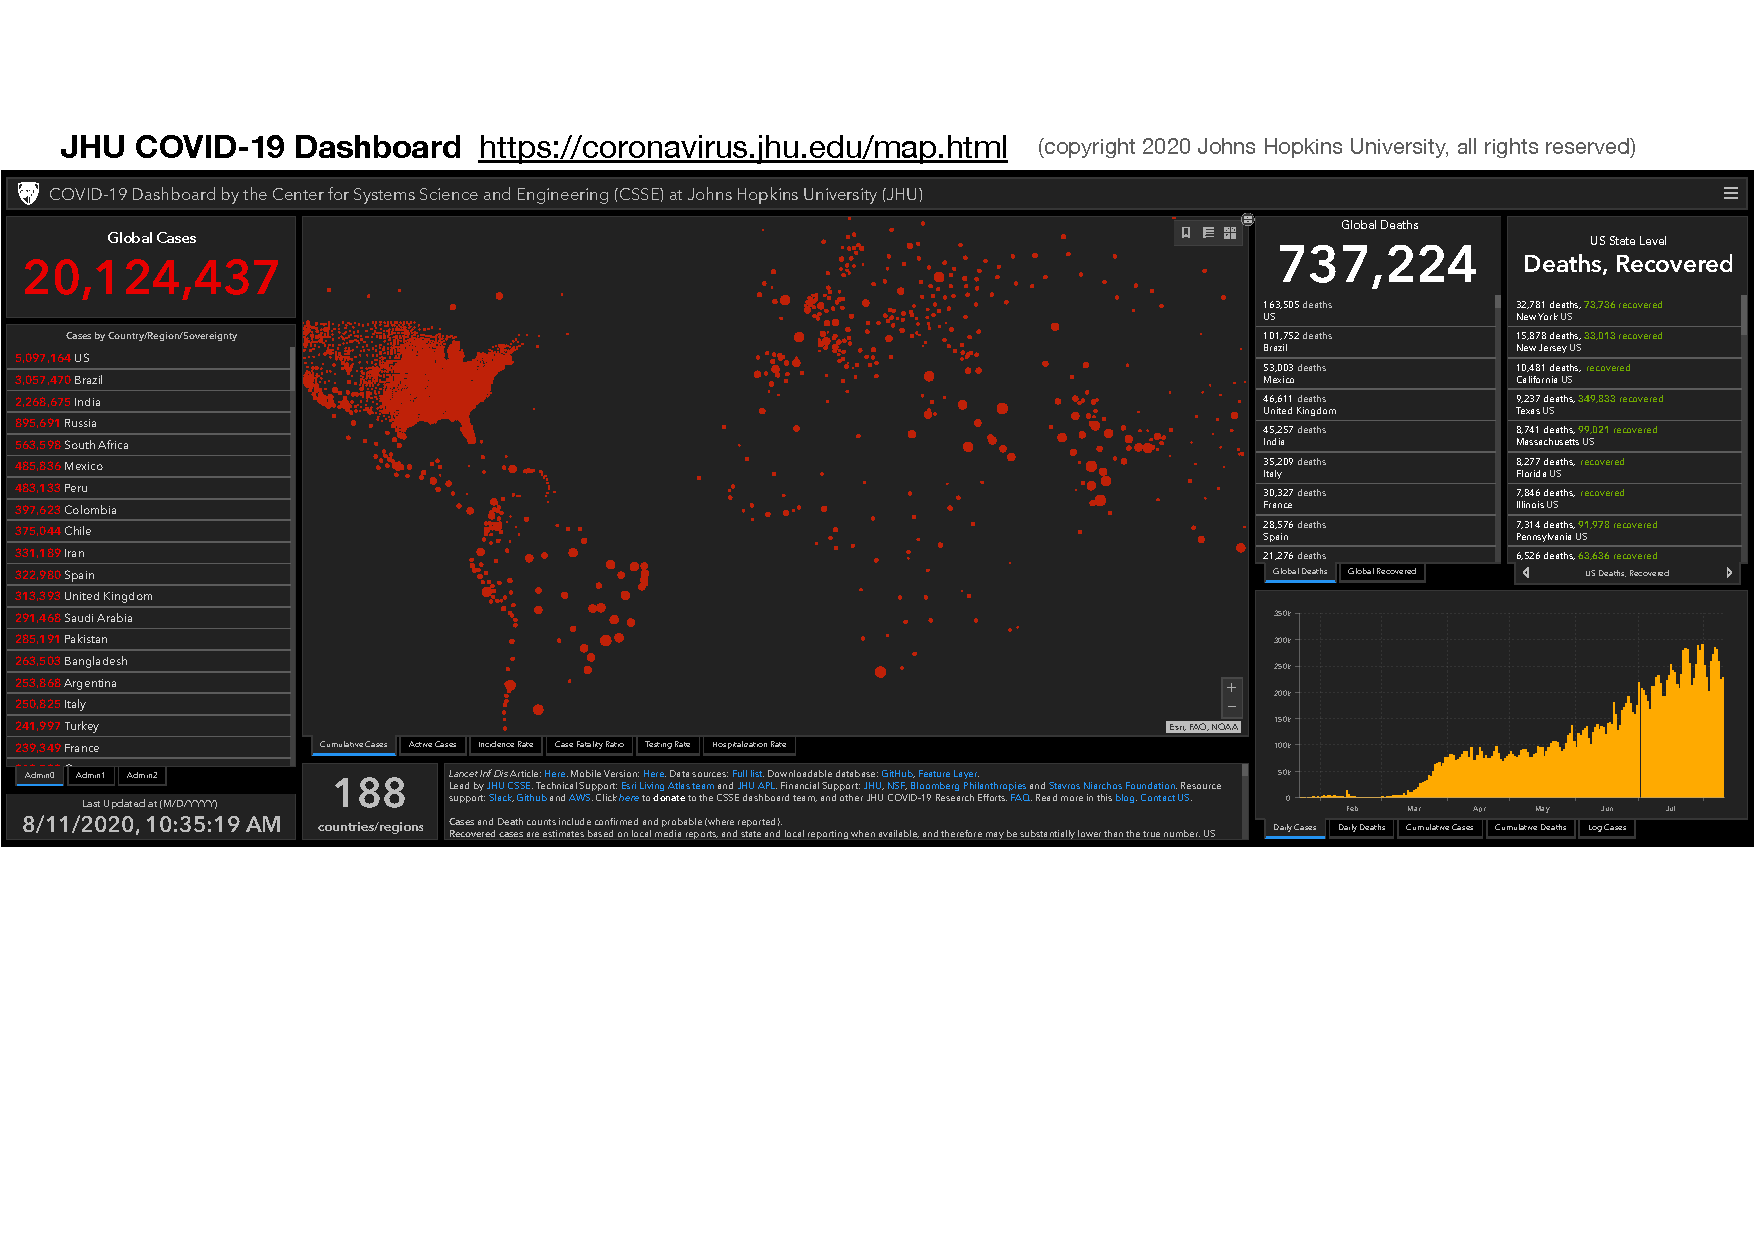
\includegraphics[width=0.95\textwidth]{figures/jhu-dashboard2.pdf}
	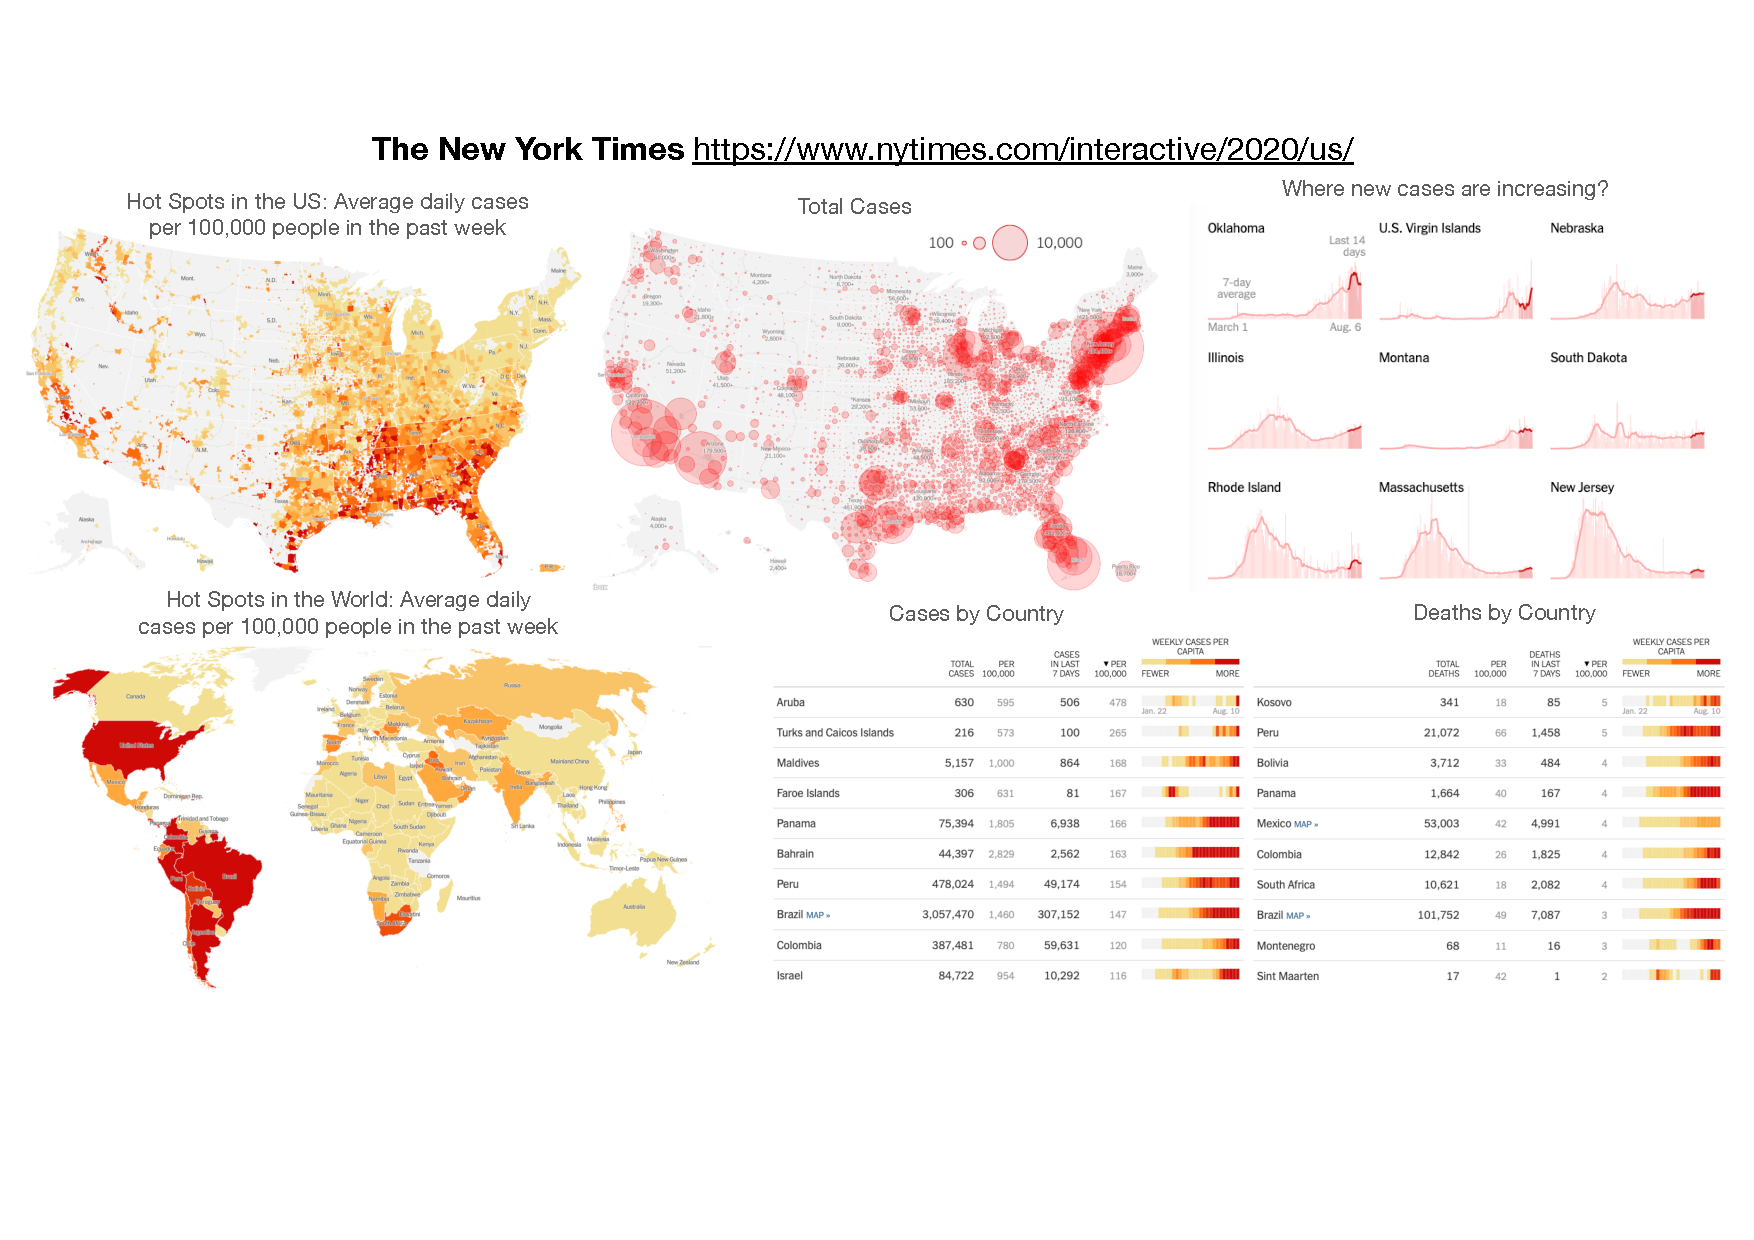
\includegraphics[width=0.95\textwidth]{figures/ny-times.pdf}
	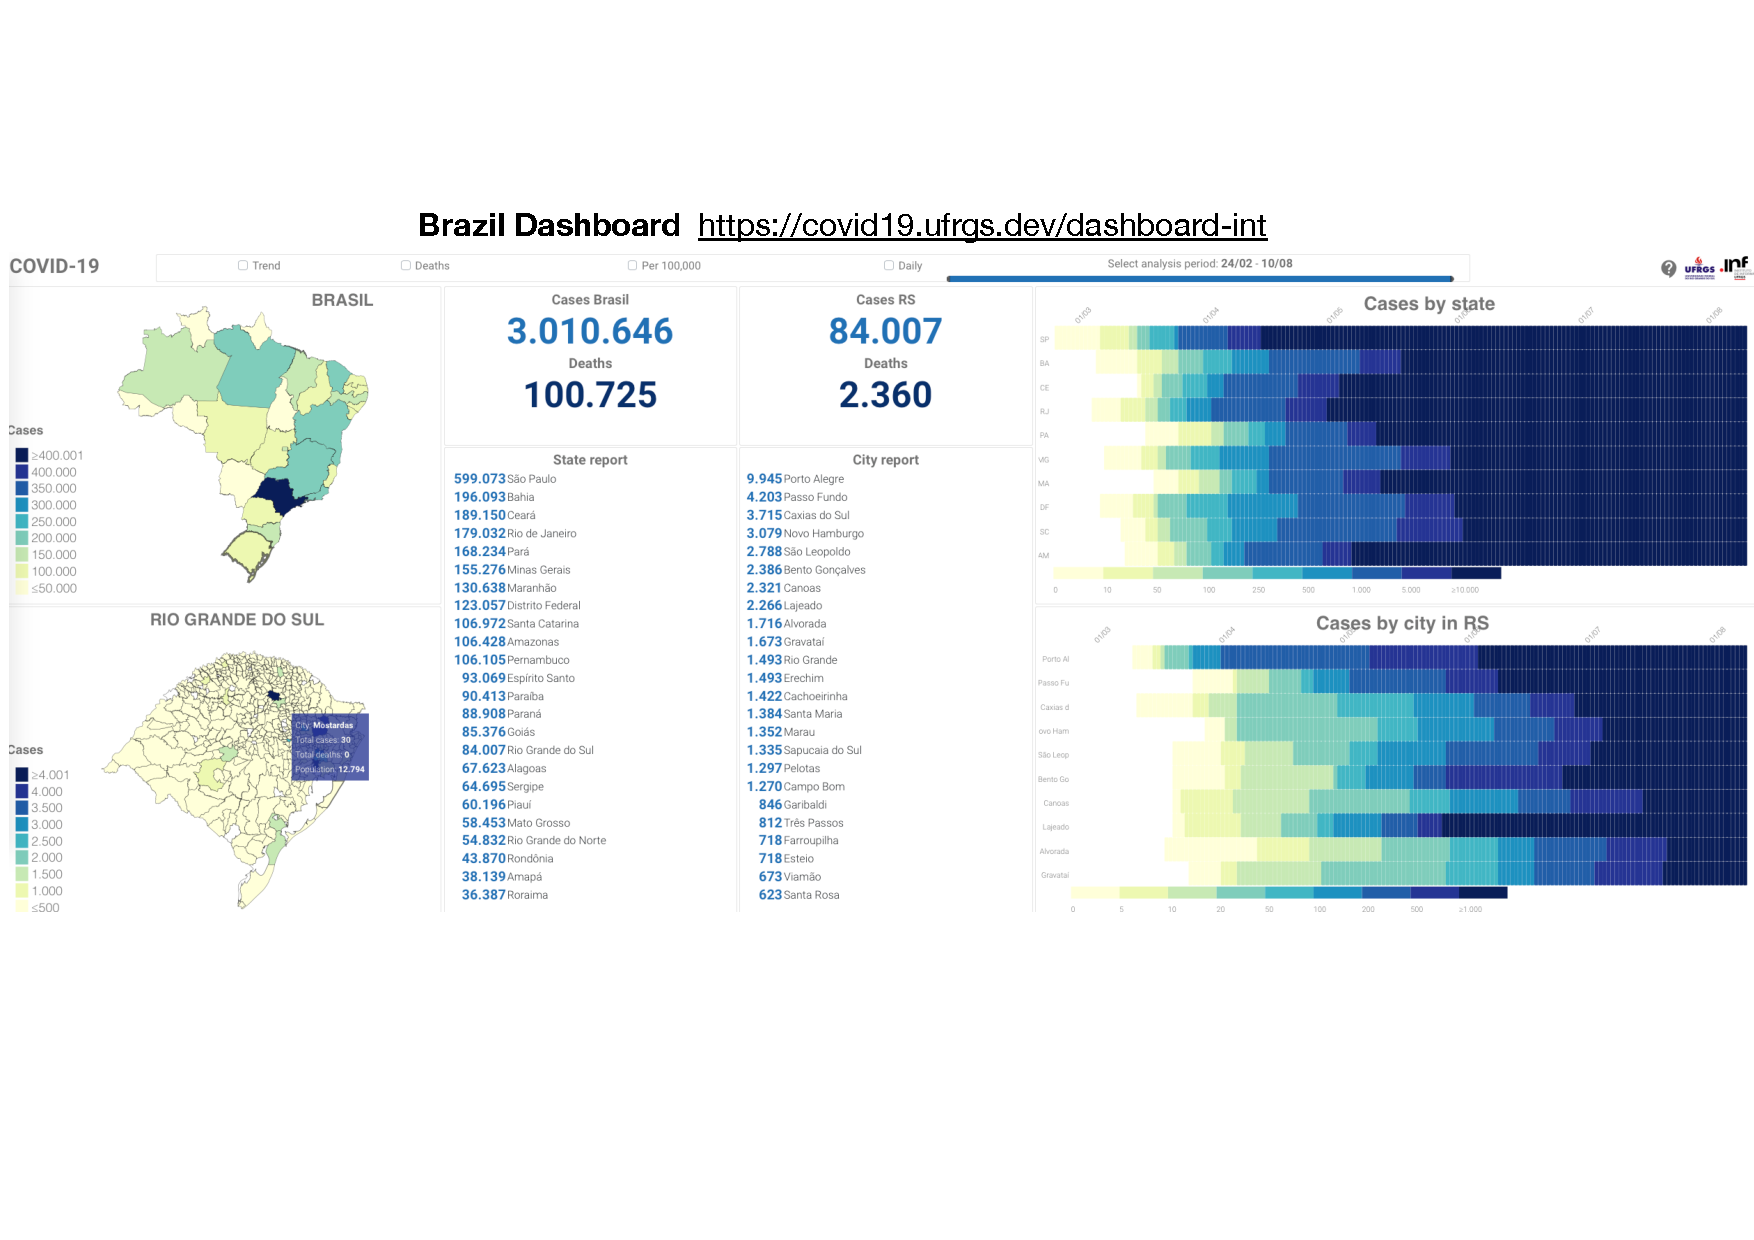
\includegraphics[width=0.95\textwidth]{figures/brazil-dashboard.pdf}
	\caption{Dashboads and interactive tools to analyse COVID-19 data: JHU Dashboard, The New York Times charts and INF-UFRGS Brazil Dashboard.}
	\label{fig:dashboards}
\end{figure*}

\begin{figure*}
	\includegraphics[width=\textwidth]{figures/chart2.pdf}
	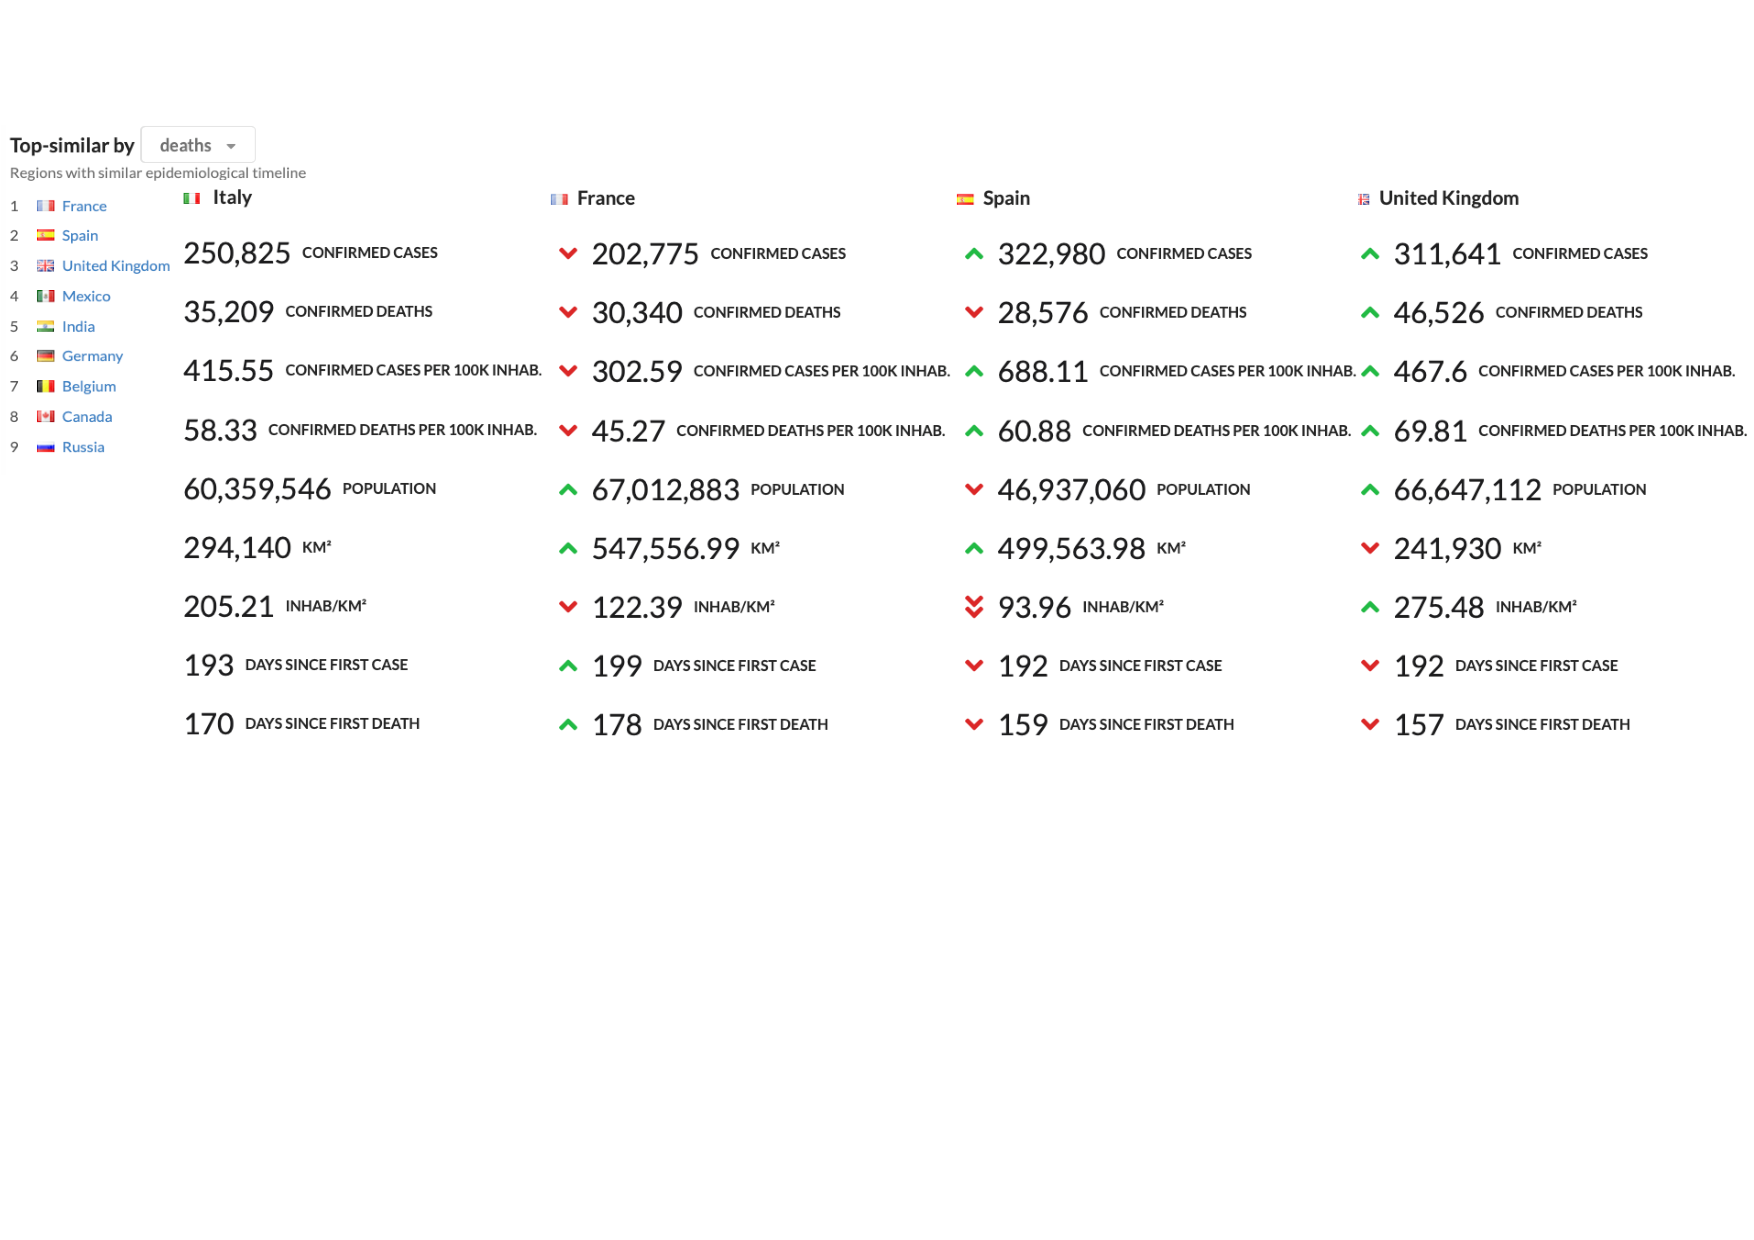
\includegraphics[width=\textwidth]{figures/similarity1.pdf}
	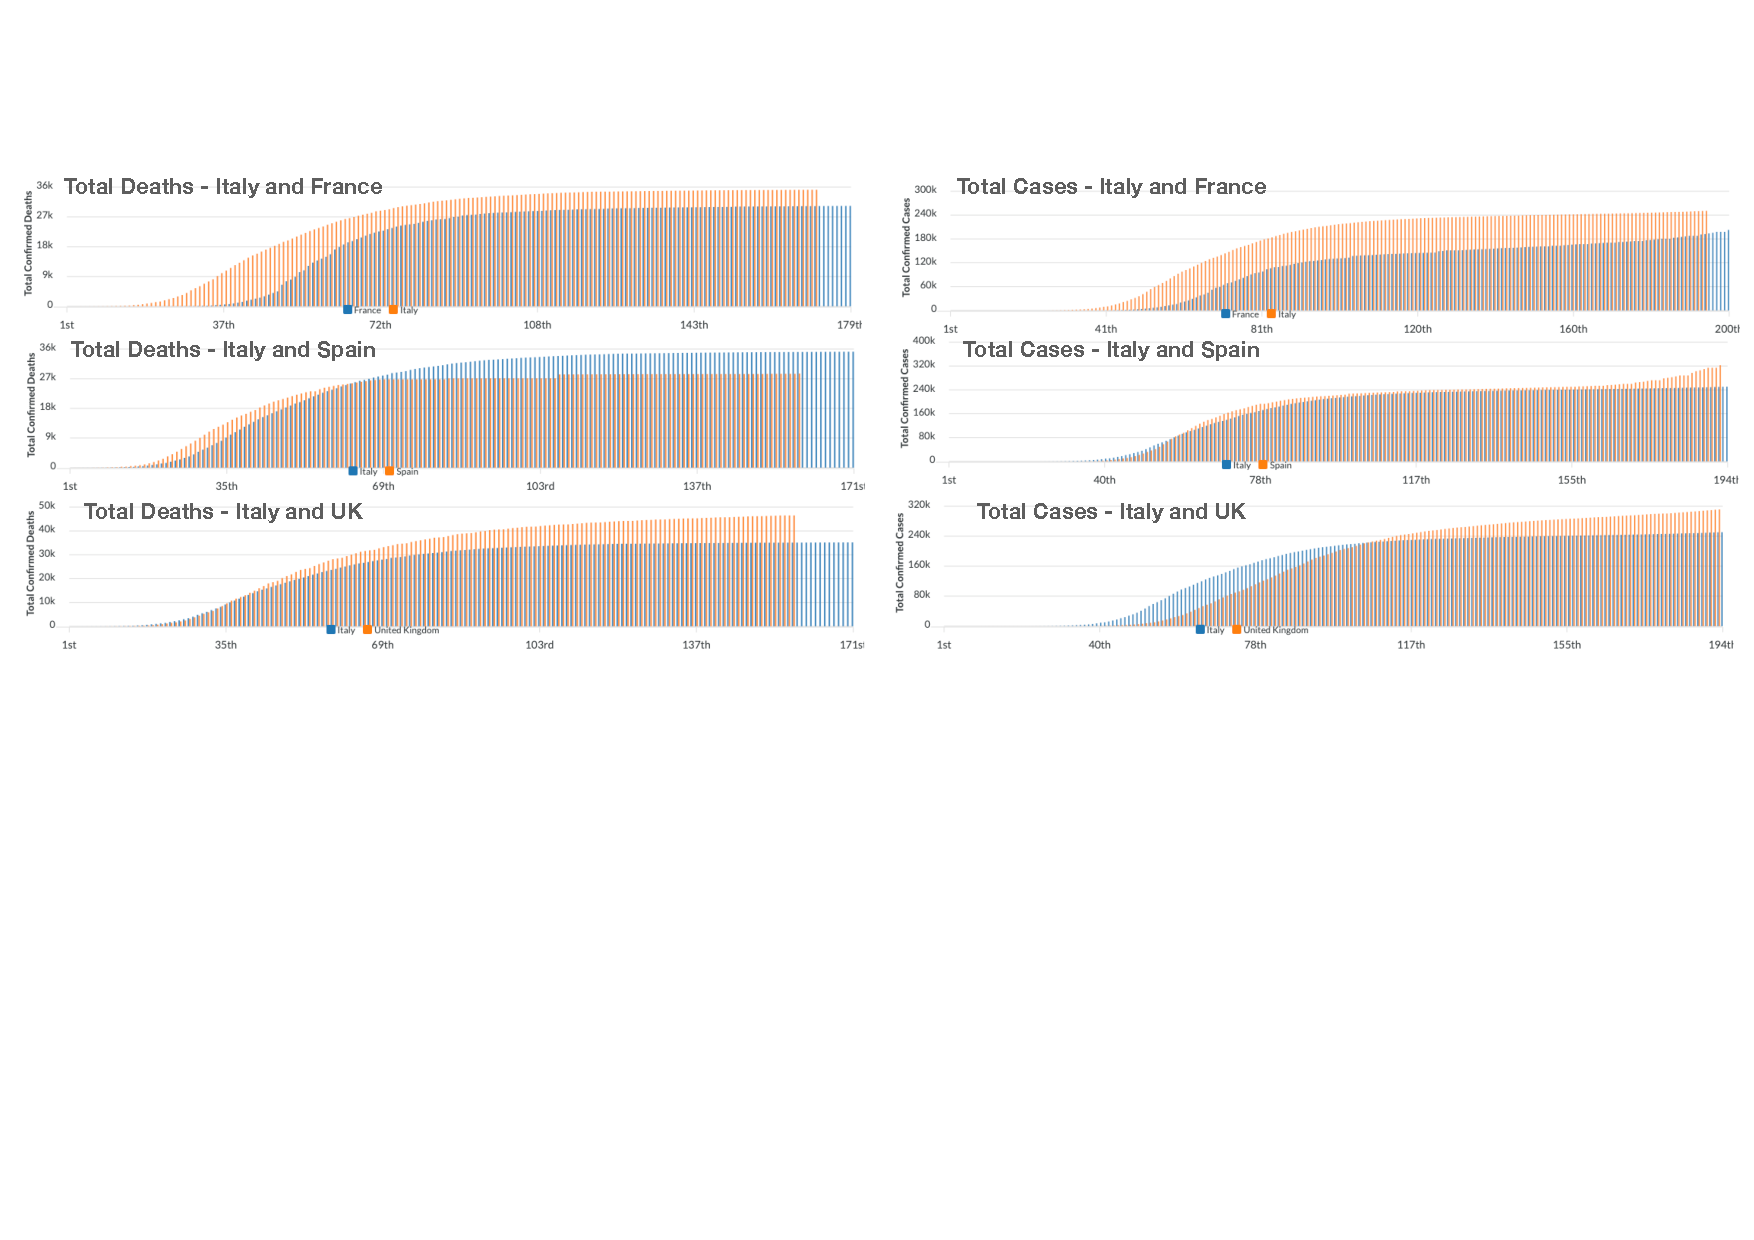
\includegraphics[width=\textwidth]{figures/similarity2.pdf}
	\caption{(top) Heatmap matrices are useful for comparing time series such as the total deaths for different countries. Columns can be aligned by the first date after reaching a certain threshold, which allows to compare when countries passed through specific checkpoints. (bottom) Searching for places with similar timelines of deaths to Italy.}
	\label{fig:covid19-tool}
\end{figure*}

\begin{figure*}
	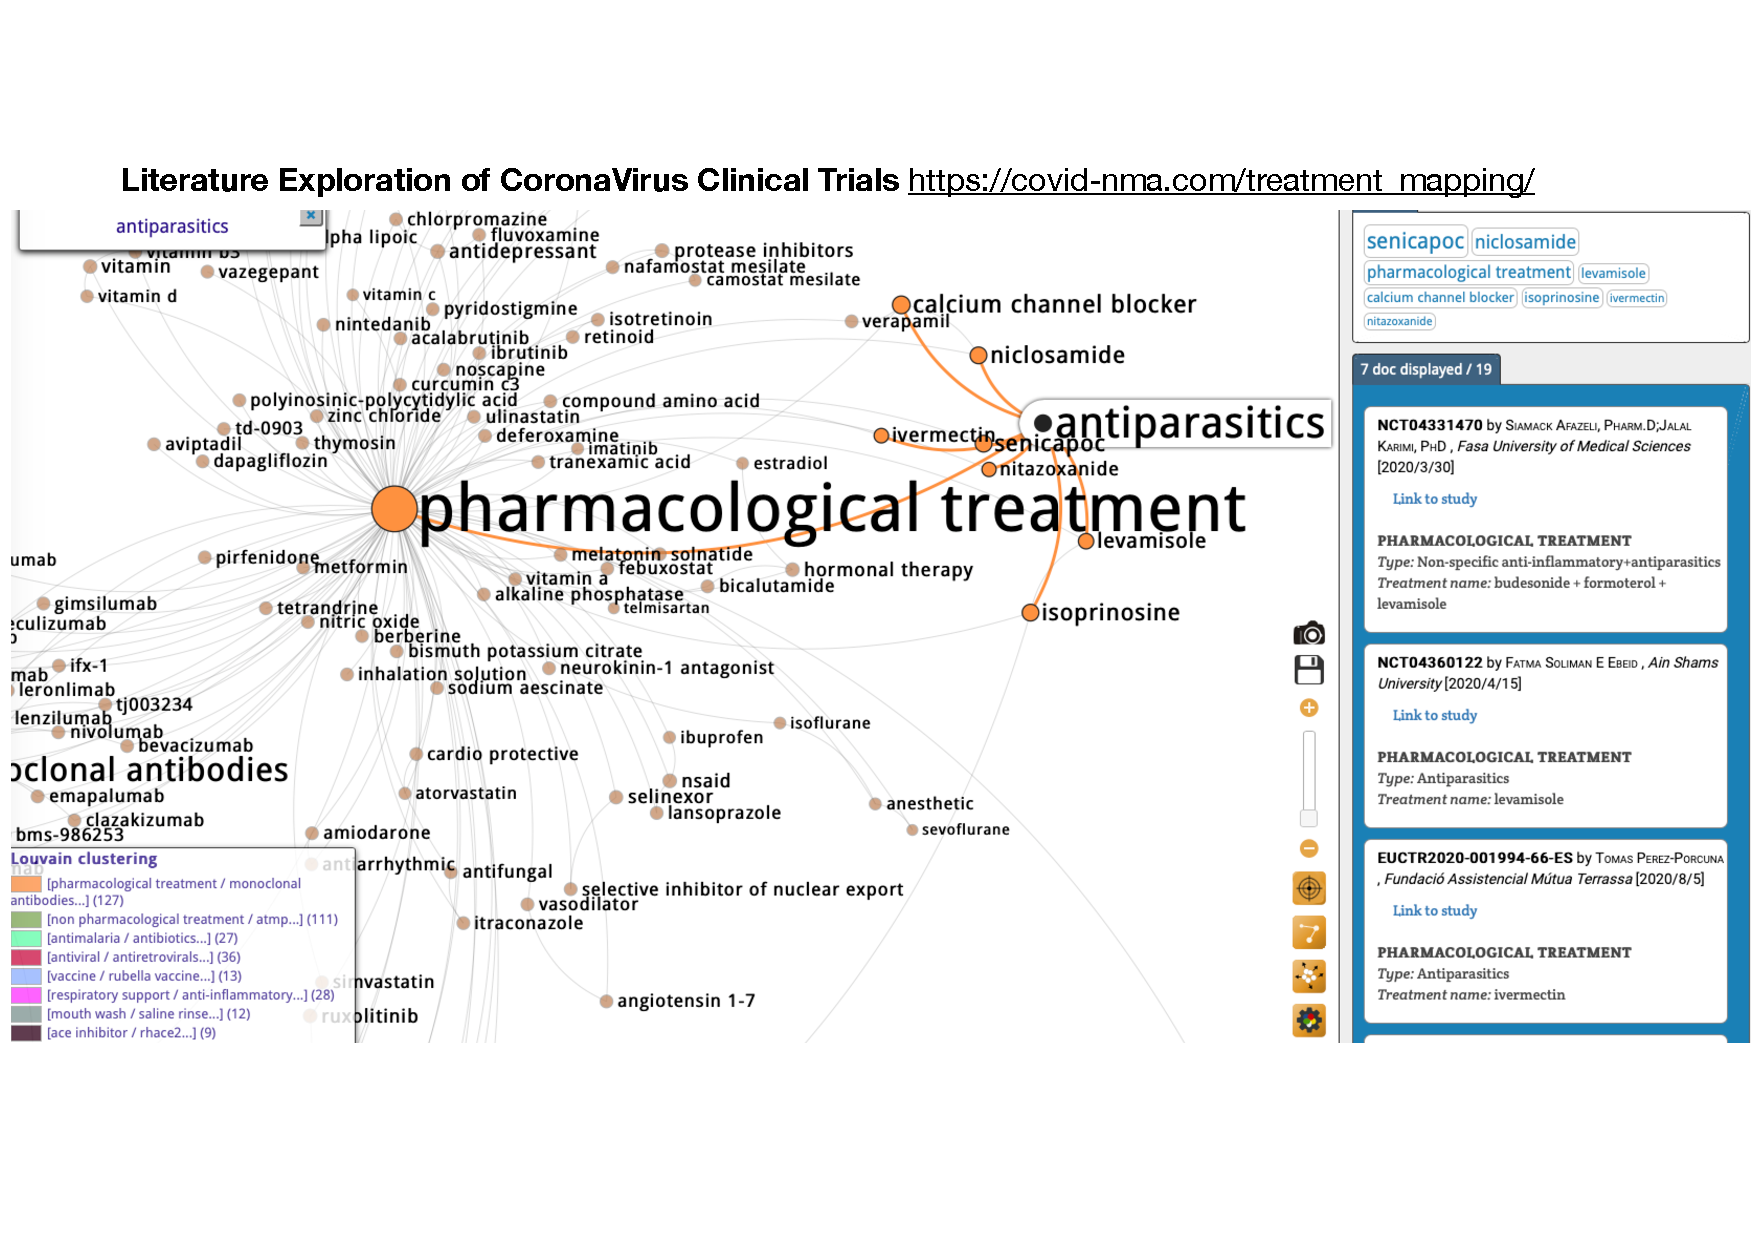
\includegraphics[width=\textwidth]{figures/applications1.pdf}
	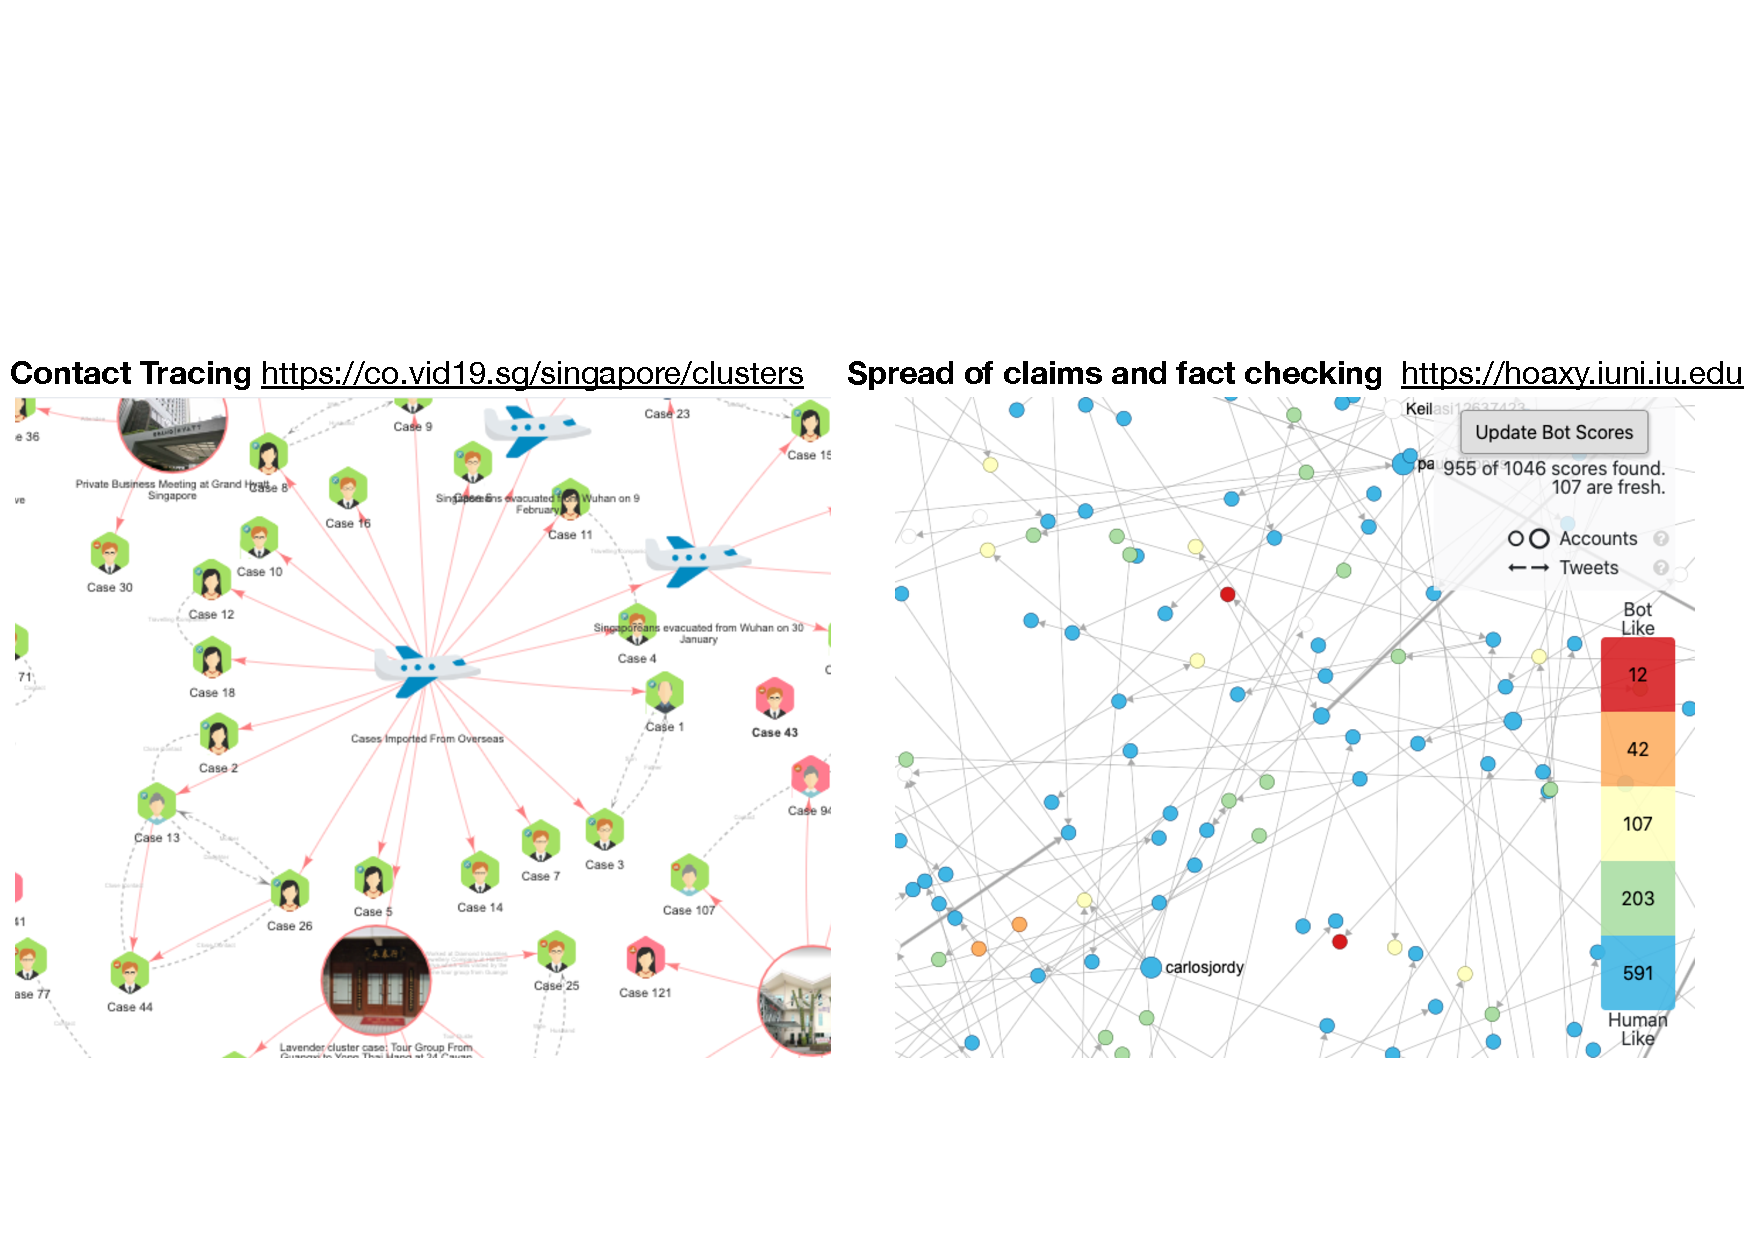
\includegraphics[width=\linewidth]{figures/applications2.pdf}
	\includegraphics[width=\linewidth]{figures/applications3.pdf}
	\caption{Applications: Literature exploration, contact tracing, spread of claims and fact checking, and simulation of the transport and spread of the novel coronavirus.}
	\label{fig:applications}
\end{figure*}



\end{document}
